\chapter{Referencias Bibliogr\'aficas}
\label{cap:refbib}

Neste trabalho, o objetivo foi desenvolver um multímetro capaz de medir tensão e corrente simultaneamente e enviar os dados para um smartphone por meio de uma conexão wifi. Considerando essa proposta, foram analisadas duas opções para servir como base: um multimedidor e um multímetro.

O multimedidor é um dispositivo geralmente trifásico, que permite a medição simultânea de tensão e corrente, exibindo as formas de onda em um display. Possui três ou mais canais simultâneos. No entanto, apresenta a limitação de possuir apenas um referencial de medição, com resolução na ordem de 1V nos modelos mais baratos e 0,1V nos modelos mais caros, repetindo-se esses valores para a resolução da corrente [CITAÇÃO]. (citar manual fluke 434)

Por outro lado, o multímetro é um dispositivo monofásico que permite a medição de apenas um canal por vez, como tensão, corrente, resistência, capacitância, entre outros. Ele não exibe as curvas na tela, fornecendo apenas os valores. A resolução varia, sendo que nos modelos mais simples pode chegar a 0,1 mV, enquanto a resolução da corrente é da ordem de 1uA [CITAÇÃO]. (Citar manual ET-1100B)

Considerando que o dispositivo deve ser utilizado como uma ferramenta didática em sala de aula, é essencial que a resolução seja adequada para o bom aproveitamento das disciplinas. Além disso, a apresentação das formas de onda também é relevante. Assim, optou-se por uma abordagem que combina características de ambos os dispositivos, utilizando os diagramas de blocos para identificar as funcionalidades e suas relações com o dispositivo a ser produzido.

Para o multimedidor, foi utilizado o diagrama de blocos do \textit{oZm3} (\autoref{fig:ozm3flowchart}), um produto \textit{open source} (projeto aberto) já introduzido no mercado, sendo uma versão trifásica de outro, também \textit{open source} chamado \textit{(openZmeter)}. Ambos possuem interface de apresentação dos dados via uma página do navegador de um celular ou computador.

\begin{figure}[h]
    \caption{Diagrama de blocos do multimedidor trifásico oZm3}
    \label{fig:ozm3flowchart}
    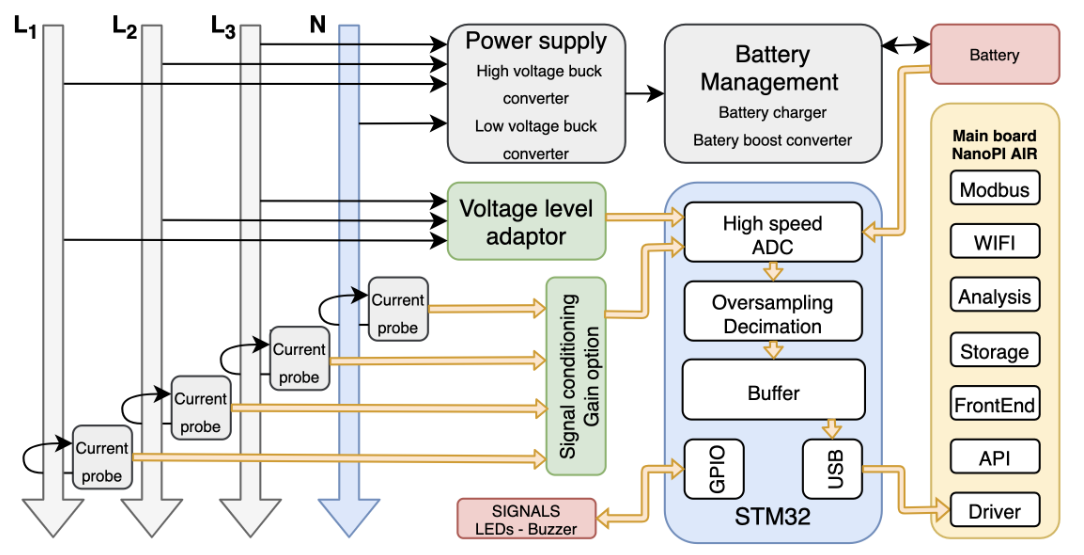
\includegraphics[width=0.8\textwidth]{figuras/openzmeter-diagrama.png}
    \fonte{CITAR Open Source Oz3.pdf}
\end{figure}

Para o multímetro, foi utilizado um diagrama de blocos (\autoref{fig:multimeterflowchart}) disponível no site da (CITAÇÃO) \textit{Texas Instruments}, que explica o funcionamento de um produto completo.

\begin{figure}[h]%% Ambiente figure
    %\captionsetup{width=0.55\textwidth}%% Largura da legenda
    \caption{Exemplo de um Diagrama de Blocos de um Multímetro}%% Legenda
    \label{fig:multimeterflowchart}%% Rótulo
    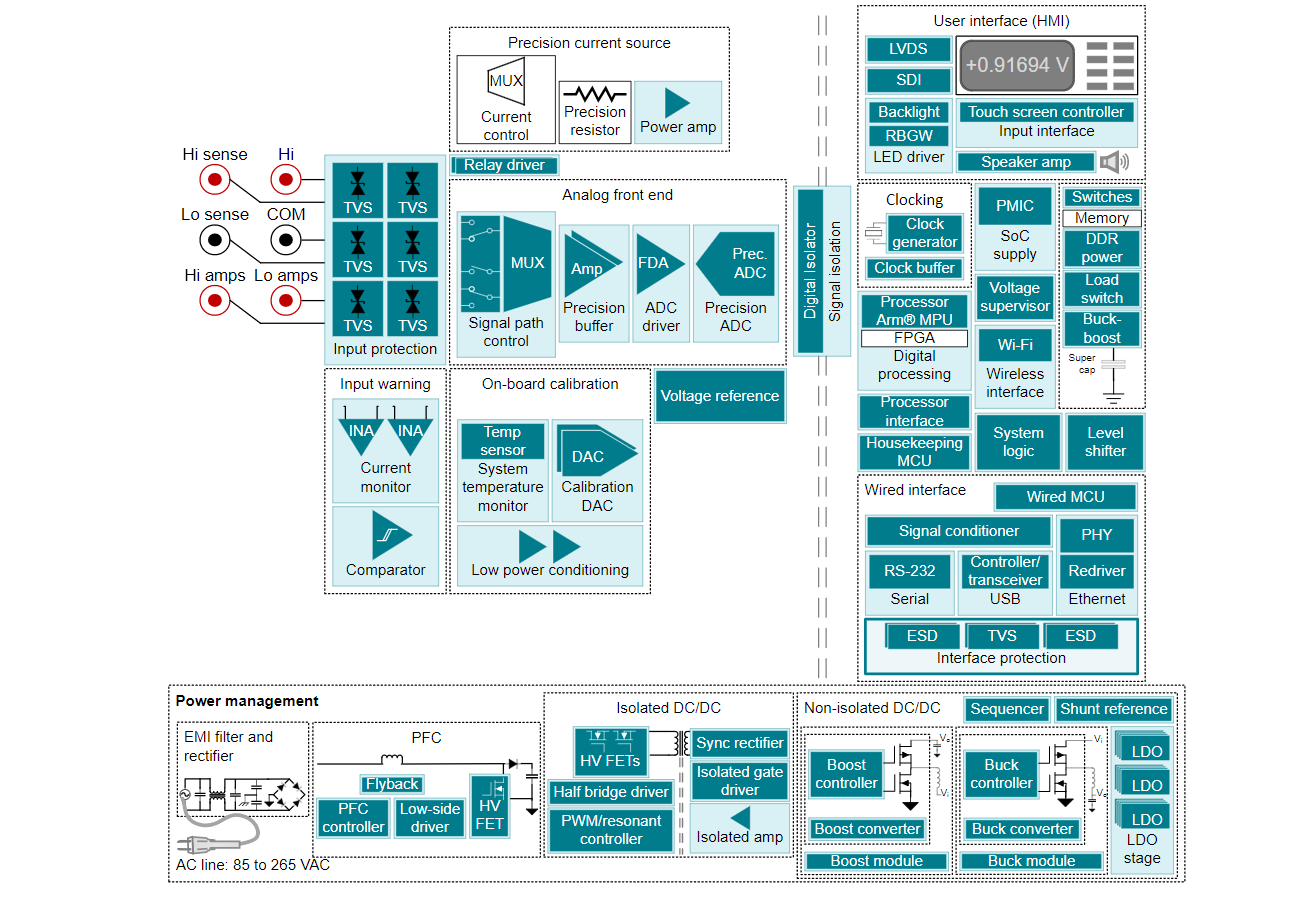
\includegraphics[width=1\textwidth]{flowchart}%% Dimensões e localização
    \fonte{Texas Instruments}%% Fonte
\end{figure}


[[ADICIONAR MAIS INFORMAÇÕES SOBRE O ESTADO DA ARTE]]
%https://www.fluke.com/en/product/intrinsically-safe/fluke-28-ii-ex (Fluke 28-II EX)
%https://www.tek.com/en/products/keithley/digital-multimeter/dmm7510 (Benchtop DMM)
%https://www.testmart.com/webdata/mfr_pdfs/FLU/27______smeng0100.pdf (Handheld, old DMM)